%%%%%%%%%%%%%%%%%%%%%%%%%%%%%%%%%%%%%%%%%
% Masters/Doctoral Thesis 
% LaTeX Template
% Version 2.5 (27/8/17)
%
% This template was downloaded from:
% http://www.LaTeXTemplates.com
%
% Version 2.x major modifications by:
% Vel (vel@latextemplates.com)
%
% This template is based on a template by:
% Steve Gunn (http://users.ecs.soton.ac.uk/srg/softwaretools/document/templates/)
% Sunil Patel (http://www.sunilpatel.co.uk/thesis-template/)
%
% Template license:
% CC BY-NC-SA 3.0 (http://creativecommons.org/licenses/by-nc-sa/3.0/)
%
%%%%%%%%%%%%%%%%%%%%%%%%%%%%%%%%%%%%%%%%%

%----------------------------------------------------------------------------------------
%	PACKAGES AND OTHER DOCUMENT CONFIGURATIONS
%----------------------------------------------------------------------------------------

\documentclass[
11pt, % The default document font size, options: 10pt, 11pt, 12pt
%oneside, % Two side (alternating margins) for binding by default, uncomment to switch to one side
french, % ngerman for German
singlespacing, % Single line spacing, alternatives: onehalfspacing or doublespacing
%draft, % Uncomment to enable draft mode (no pictures, no links, overfull hboxes indicated)
%nolistspacing, % If the document is onehalfspacing or doublespacing, uncomment this to set spacing in lists to single
%liststotoc, % Uncomment to add the list of figures/tables/etc to the table of contents
%toctotoc, % Uncomment to add the main table of contents to the table of contents
%parskip, % Uncomment to add space between paragraphs
%nohyperref, % Uncomment to not load the hyperref package
headsepline, % Uncomment to get a line under the header
%chapterinoneline, % Uncomment to place the chapter title next to the number on one line
%consistentlayout, % Uncomment to change the layout of the declaration, abstract and acknowledgements pages to match the default layout
]{MastersDoctoralThesis} % The class file specifying the document structure

\usepackage[utf8]{inputenc} % Required for inputting international characters
\usepackage[T1]{fontenc} % Output font encoding for international characters
\usepackage{xparse}
\usepackage{mathpazo} % Use the Palatino font by default

\usepackage[backend=bibtex,style=authoryear,natbib=true]{biblatex} % Use the bibtex backend with the authoryear citation style (which resembles APA)

\addbibresource{example.bib} % The filename of the bibliography

\usepackage[autostyle=true]{csquotes} % Required to generate language-dependent quotes in the bibliography
\usepackage{enumitem} % package for enumeration with bullet in french
\usepackage{float} % package for the float objects
\usepackage{graphicx}
\usepackage{lscape}
\usepackage{xparse}

\usepackage[most]{tcolorbox}

\tcbset
{
    frame code={}
    center title,
    left=0pt,
    right=0pt,
    top=0pt,
	bottom=0pt,
	colupper=white,
    colback=black,
    colframe=white,
    width=\dimexpr\textwidth\relax,
    enlarge left by=0mm,
    boxsep=3pt,
	arc=0pt,outer arc=0pt,
	halign=left,
}

\ExplSyntaxOn
\NewDocumentCommand{\tabhead}{ O{\bfseries} m }
 {
  \seq_set_split:Nnn \l_tmpa_seq { & } { #2 }
  #1 \seq_use:Nn \l_tmpa_seq { & #1 } \\
 }
\ExplSyntaxOff

\let\cleardoublepage\clearpage

\usepackage{inconsolata}
\usepackage{color}
\usepackage{listings}
\usepackage{textcomp}

%----------------------------------------------------------------------------------------
%	FOR THE LIST OF EQUATIONS
%----------------------------------------------------------------------------------------
\usepackage{tocloft}
\usepackage{xstring}
%\makeatletter

% we use this for our refernces as well
%\AtBeginDocument{\renewcommand{\ref}[1]{\mbox{\autoref{#1}}}}

% redefinition of \equation for convenience
%\let\oldequation = \equation
%\let\endoldequation = \endequation
%\AtBeginDocument{\let\oldlabel = \label}% \AtBeginDocument because hyperref redefines \label
%\newcommand{\mynewlabel}[1]{%
%  \StrBehind{#1}{eq:}[\Str]% remove "eq:" from labels
%  \myequations{\Str}\oldlabel{#1}}
 % \renewenvironment{equation}{%
 % \oldequation
 % \let\label\mynewlabel
%}{\endoldequation}

%\newcommand{\listequationsname}{Liste des équations}
%\newlistof{myequations}{equ}{\listequationsname}
%\newcommand{\myequations}[1]{%
%      \addcontentsline{equ}{myequations}{\protect\numberline{\theequation}#1}}
%	  \setlength{\cftmyequationsindent}{1.5em}
%	  \setlength{\cftmyequationsnumwidth}{2.3em}

%\makeatother

\lstset
{
   	language=bash, %% Troque para PHP, C, Java, etc... bash é o padrão
   	basicstyle=\ttfamily\small,
   	numberstyle=\footnotesize,
   	numbers=left,
   	backgroundcolor=\color{gray!10},
   	frame=single,
   	tabsize=2,
   	rulecolor=\color{black!30},
   	title=\lstname,
    escapeinside={\%*}{*)},
    breaklines=true,
    breakatwhitespace=true,
    %framextopmargin=0pt,
    %framexbottommargin=0pt,
    inputencoding=utf8,
    extendedchars=true,
    literate={á}{{\'a}}1 {ã}{{\~a}}1 {é}{{\'e}}1,
}

%----------------------------------------------------------------------------------------
%	MARGIN SETTINGS
%----------------------------------------------------------------------------------------

\geometry{
	paper=a4paper, % Change to letterpaper for US letter
	inner=2.5cm, % Inner margin
	outer=3.8cm, % Outer margin
	bindingoffset=.5cm, % Binding offset
	top=1.5cm, % Top margin
	bottom=1.5cm, % Bottom margin
	%showframe, % Uncomment to show how the type block is set on the page
}

%----------------------------------------------------------------------------------------
%	THESIS INFORMATION
%----------------------------------------------------------------------------------------

\thesistitle{Intégration du driver IMX219 sur une OpenRex Basic} % Your thesis title, this is used in the title and abstract, print it elsewhere with \ttitle
\supervisor{Patrick \textsc{Piquart} \\
			David \textsc{Coué}} % Your supervisor's name, this is used in the title page, print it elsewhere with \supname
\examiner{} % Your examiner's name, this is not currently used anywhere in the template, print it elsewhere with \examname
\degree{Master Systèmes Embarqués} % Your degree name, this is used in the title page and abstract, print it elsewhere with \degreename
\author{Alan \textsc{Ait-Ali}, Martin \textsc{Laporte}, \\
Clément \textsc{Ailloud} \& Romain \textsc{Petit} \\ } % Your name, this is used in the title page and abstract, print it elsewhere with \authorname
\addresses{} % Your address, this is not currently used anywhere in the template, print it elsewhere with \addressname

\subject{Biological Sciences} % Your subject area, this is not currently used anywhere in the template, print it elsewhere with \subjectname
\keywords{} % Keywords for your thesis, this is not currently used anywhere in the template, print it elsewhere with \keywordnames
\university{YNOV} % Your university's name and URL, this is used in the title page and abstract, print it elsewhere with \univname
\department{Département Aéronautique \& Systèmes Embarqués} % Your department's name and URL, this is used in the title page and abstract, print it elsewhere with \deptname
\group{Département Aéronautique \& Systèmes Embarqués} % Your research group's name and URL, this is used in the title page, print it elsewhere with \groupname
\faculty{YNOV} % Your faculty's name and URL, this is used in the title page and abstract, print it elsewhere with \facname

\AtBeginDocument{
\hypersetup{pdftitle=\ttitle} % Set the PDF's title to your title
\hypersetup{pdfauthor=\authorname} % Set the PDF's author to your name
\hypersetup{pdfkeywords=\keywordnames} % Set the PDF's keywords to your keywords
}

\begin{document}

\frontmatter % Use roman page numbering style (i, ii, iii, iv...) for the pre-content pages

\pagestyle{plain} % Default to the plain heading style until the thesis style is called for the body content

%----------------------------------------------------------------------------------------
%	TITLE PAGE
%----------------------------------------------------------------------------------------

\begin{titlepage}
\begin{center}

\vspace*{.06\textheight}
{\scshape\LARGE \univname\par}\vspace{1.5cm} % University name
\textsc{\Large Projet de Master en partenariat avec Thales}\\[0.5cm] % Thesis type

\HRule \\[0.4cm] % Horizontal line
{\huge \bfseries \ttitle\par}\vspace{0.4cm} % Thesis title
\HRule \\[1.5cm] % Horizontal line
 
\begin{minipage}[t]{0.4\textwidth}
\begin{flushleft} \large
\emph{Auteur :}\\
Alan \textsc{Ait-Ali} \\
Martin \textsc{Laporte} \\
Clément \textsc{Ailloud} \\
Romain \textsc{Petit}
%\authorname % Author name - remove the \href bracket to remove the link
\end{flushleft}
\end{minipage}
\begin{minipage}[t]{0.4\textwidth}
\begin{flushright} \large
\emph{Superviseurs :} \\
\supname % Supervisor name - remove the \href bracket to remove the link  
\end{flushright}
\end{minipage}\\[3cm]

\large \textit{Rapport final présentant le travail effectué sur \\
				l'intégration du driver IMX219 sur une OpenRex Basic}\\[0.3cm] % University requirement text
\textit{au sein du}\\[0.4cm]
\deptname\\[2cm] % Research group name and department name


\includegraphics[scale=0.7]{/home/romain/Pictures/Logo_Ynov.png}\\[1cm] % University/department logo - uncomment to place it

{\large \today}\\[4cm] % Date

 
\vfill
\end{center}
\end{titlepage}

%----------------------------------------------------------------------------------------
%	DECLARATION PAGE
%----------------------------------------------------------------------------------------

%\begin{declaration}
%\addchaptertocentry{\authorshipname} % Add the declaration to the table of contents
%\noindent Je, \authorname, declare que ce mémoire intitulé, \enquote{\ttitle} et le travail qui y est présenté, est le mien. Je confirme que :

%\begin{itemize}[label=$\bullet$] 
%\item Ce travail a été réalisé entièrement ou principalement pour l'obtention de mon diplôme au sein de l'école E.S.T.E.I.
%\item Si une partie quelconque de cette thèse a déjà été soumise pour obtenir un diplôme ou toute autre qualification dans cette école ou dans une autre institution, cela est clairement indiqué.
%\item Lorsque je consulte le travail publié d'autrui, cela est toujours clairement attribué.
%\item Lorsque je cite le travail des autres, la source est toujours donnée. À l'exception de ces citations, cette thèse est entièrement mon propre travail.
%\item J'ai pris connaissances de toutes les principales sources d'aide.
%\item Lorsque la thèse est basée sur le travail effectué par moi-même conjointement avec d'autres, j'ai précisé exactement ma contribution et ce qui a été fait par les autres.\\
%\end{itemize}
 
%\noindent Signature:\\
%\rule[0.5em]{25em}{0.5pt} % This prints a line for the signature
 
%\noindent Date:\\
%\rule[0.5em]{25em}{0.5pt} % This prints a line to write the date
%\end{declaration}

%\cleardoublepage

%----------------------------------------------------------------------------------------
%	QUOTATION PAGE
%----------------------------------------------------------------------------------------

%\vspace*{0.2\textheight}

%\noindent\enquote{\itshape Thanks to my solid academic training, today I can write hundreds of words on virtually any topic without possessing a shred of information, which is how I got a good job in journalism.}\bigbreak

%\hfill Dave Barry

%----------------------------------------------------------------------------------------
%	ABSTRACT PAGE
%----------------------------------------------------------------------------------------

\begin{abstract}
\addchaptertocentry{\abstractname} % Add the abstract to the table of contents

Actuellement, les casques de réalité augmentée pour pilote migrent vers le domaine civil. Thales a
réalisé un prototype fonctionnant avec une Raspberry Pi et la Raspberry Pi Camera pour 
l’acquisition d’images ou de flux vidéo. Thales a fait appel aux étudiants du campus Ynov pour 
participer à l’amélioration de ce prototype. 

L’objectif du projet est de réaliser le portage du driver de la caméra sur un autre système 
d’exploitation que Raspberry Pi. Ce système devra donc être capable faire des captures d’image et un
flux vidéo de la caméra depuis une autre carte, l’Openrex-IMX6-Quad car pour des raisons internes à 
l’équipe de développement Thales-LUCY.

Avec Yocto, nous avons généré dans un premier temps, un système d’exploitation fonctionnel sur la 
carte cible (kernel Linux 3.14 puis 4.1). Par la suite, nous avons essayé de faire fonctionner des
codes existants en les adaptant à la carte Openrex. N’y arrivant pas, nous avons alors entrepris la
rédaction d’un driver de la caméra. Actuellement, nous avons réussi à établir une connexion I2C entre
la caméra et l’IMX6 Openrex en utilisant le port CSI-2.

Notre travail étant inachevé, ce rapport permet de partager nos connaissances acquises lors du 
déroulement du projet. Il est nécessaire pour une bonne compréhension d’être introduit à l’usage de 
Yocto. \bigskip

Nowadays augmented reality pilot’s helmet move to the civil domain. At the moment Thales group 
prototyped one working with a Raspberry Pi and it’s associated raspberry camera v2 for picture and
video capture. Thales called ynov campus students for applications at being part of the prototype
improvement. 

Our aim is to build an Raspberry Pi camera, picture and video capture compatible, operating system 
on l’Openrex-IMX6-Quad. Indeed for Thales-LUCY team internal reasons the initial Raspberry Pi board 
won’t be used in the MVP project state.

In a first hand we built a Yocto-project generated target board operating system (kernel Linux 3.14 
then 4.1). In a second hand we tried to port existing source codes to the Openrex board. Unable to 
succeed, we undertook the camera driver redaction from scratch. We already connected the camera 
module with both CSI and I2C communication protocols as the mobile industry processor interface 
(MIPI) standard describes.

As our work in unfinished, the present report hand our state of knowledge and achievement over. 
Linux operating system Yocto generation usage knowledge is needed for it’s good understanding.

%\ldots
\end{abstract}

%----------------------------------------------------------------------------------------
%	ACKNOWLEDGEMENTS
%----------------------------------------------------------------------------------------

\begin{acknowledgements}
\addchaptertocentry{\acknowledgementname} % Add the acknowledgements to the table of contents
Les remerciements et les personnes à remercier vont ici, n'oubliez pas d'inclure vos conseillers de projets et superviseurs\ldots
\end{acknowledgements}

%----------------------------------------------------------------------------------------
%	LIST OF CONTENTS/FIGURES/TABLES PAGES
%----------------------------------------------------------------------------------------

\tableofcontents % Prints the main table of contents
\clearpage

\listoffigures % Prints the list of figures
\clearpage

\listoftables % Prints the list of tables
\clearpage

%\listofmyequations


%----------------------------------------------------------------------------------------
%	ABBREVIATIONS
%----------------------------------------------------------------------------------------

%\begin{abbreviations}{ll} % Include a list of abbreviations (a table of two columns)

%\textbf{LAH} & \textbf{L}ist \textbf{A}bbreviations \textbf{H}ere\\
%\textbf{WSF} & \textbf{W}hat (it) \textbf{S}tands \textbf{F}or\\

%\end{abbreviations}

%----------------------------------------------------------------------------------------
%	PHYSICAL CONSTANTS/OTHER DEFINITIONS
%----------------------------------------------------------------------------------------

%\begin{constants}{lr@{${}={}$}l} % The list of physical constants is a three column table

% The \SI{}{} command is provided by the siunitx package, see its documentation for instructions on how to use it

%Speed of Light & $c_{0}$ & \SI{2.99792458e8}{\meter\per\second} (exact)\\
%Constant Name & $Symbol$ & $Constant Value$ with units\\

%\end{constants}

%----------------------------------------------------------------------------------------
%	SYMBOLS
%----------------------------------------------------------------------------------------

%\begin{symbols}{lll} % Include a list of Symbols (a three column table)

%$a$ & distance & \si{\meter} \\
%$P$ & power & \si{\watt} (\si{\joule\per\second}) \\
%Symbol & Name & Unit \\

%\addlinespace % Gap to separate the Roman symbols from the Greek

%$\omega$ & angular frequency & \si{\radian} \\

%\end{symbols}

%----------------------------------------------------------------------------------------
%	DEDICATION
%----------------------------------------------------------------------------------------

%\dedicatory{For/Dedicated to/To my\ldots} 

%----------------------------------------------------------------------------------------
%	THESIS CONTENT - CHAPTERS
%----------------------------------------------------------------------------------------

\mainmatter % Begin numeric (1,2,3...) page numbering

\pagestyle{thesis} % Return the page headers back to the "thesis" style

% Include the chapters of the thesis as separate files from the Chapters folder
% Uncomment the lines as you write the chapters

% Chapter 1

\chapter{Organisation de l'équipe et planning} % Main chapter title

\label{Chapter1} % For referencing the chapter elsewhere, use \ref{Chapter1}

%----------------------------------------------------------------------------------------

\section{Organisation de l'équipe}

Après notre entrevue, nous avons décidé de nous séparer en deux groupes un qui
partirait du haut niveau et un autre qui partirait du bas niveau. Le but de
cette méthode est de pouvoir mieux appréhender les différents problèmes et axes
de développement. 

Le binôme Clément \& Romain recherche à faire le lien depuis
les couches applicatives vers le kernel. Le binôme Alan \& Martin au contraire
cherche à établir en priorité les couches basses pour ensuite les rendre
compatible avec le kernel.

Pour résumer les deux binômes n’ont pas le même point de départ tout en ayant la même version du kernel.

Clément et Romain sont donc chargés de l’utilisation de Gstreamer et de la
couche V4L alors que Martin et Alan sont chargés de rendre les drivers
compatibles avec notre système.

\section{Planning}

Nous vous avons ici présenté un planning des tâches effectuées durant ces 8 \\
derniers jours, les noms attribués à chaque tâche seront développés dans la suite du rapport.

\begin{figure}[th]
    \centering
    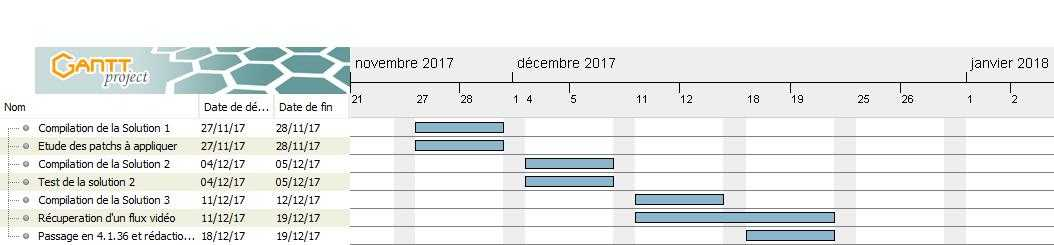
\includegraphics[width=1\linewidth]{planning.png}
    \decoRule
    \caption{Avancement du projet actuel}  \label{fig:planning}
\end{figure}

Les trois solutions qui sont présentées ci-dessous correspondent à trois codes sources.

%----------------------------------------------------------------------------------------

% Chapter 2
\chapter{Piste n° 1} % Main chapter title
\label{Chapter2} % For referencing the chapter elsewhere, use \ref{Chapter2}
%----------------------------------------------------------------------------------------

\begin{description}
  \item[Version du Kernel :] 3.14
  \item[Code de travail :] imx219.c (fichier de la solution 2 sur le rapport du
  09/01/2017)
\end{description}

Suite à l'exploration de 3 pistes de solutions, nous avons choisi de nous
concentrer sur la solutions n°2 dont le driver compile sans erreur mais ne
réussit pas le chargement en module dans le kernel.

\section{Erreur}
Constat : chargé, le driver apparait à la commande lsmod mais inutilisé.

\begin{lstlisting}
#écoute du kernel
dmesg|tail
#chargement
modprobe imx219
#écoute du kernel
dmesg|tail
\end{lstlisting}
Après recherche d'indices pour le debug, on retient un message d'erreur dans ----.
Signification incomprise correctement par recherche web, nous nous penchons donc
sur le code C. Résultat de l'annalyse :
l'erreur provient des premières lignes de la première fonction du driver. La
sécurité testant le premier paramètre d'appel du driver s'est déclanchée. le
paramètre est une structure identifiante du kernel donnée par le kernel au
driver. Il y a donc problème de compatibilité entre driver et kernel. Selon
l'avis de notre professeur de yocto qui a été appuyé par nos recherches,
le driver en question utilise les interfaces de fonctionnement nommées
platform\_data, technologie remplacée progressivement depuis 2011 par le
device-tree et sa gestion des compatibilités.

\section{Solution}
Aujourd'hui mardi 16 janvier nous avons encore cherché à porter le driver vers
une compatibilité avec le device-tree.
\begin{description}
  \item[ajout de la structure type of\_device\_id dans le driver ] ilhbce
  \begin{lstlisting}
  static const struct of\_device\_id imx6s-openrex-dt-ids[]={
    { .compatible = "imx6s , imx219-i2c",
    .data = &imx219-i2c\_config /*, sentinel*/
    },{
      /*.compatible = "",
      .data = "", sentinel*/
      },
    };
    \end{lstlisting}
    \item[Completion de la structure de manipulation du driver:] efzecr
    \begin{lstlisting}
    static const struct of_device_id imx6s-openrex-dt-ids[]={
      static struct i2c_driver imx219_i2c_driver = {
    .driver = {
      .name = "imx219",
      .of_mach_table = of_mach_ptr(imx6s-openrex-dt-ids),
      },
  	.probe = imx219_probe,
    .remove = imx219_remove,
    .id_table = imx219_id,
  };
      \end{lstlisting}
    \end{description}

    \begin{lstlisting}

    \end{lstlisting}

    \clearpage

    Inclusion des 6 dossiers de librairies en option puis nouvelles dépendances
    inexistantes dans le dossier contenant l’arborescence de compilation (builddir).
    Recherche d’une autre solution grâce au dialogue avec le professeur de Linux
    embarqué. Conseil retenu : Compilation dans l’arborescence Yocto (in-tree)
    directe. Certains fichiers restent inexistants dans le kernel 3.14 donc,
    patch depuis le kernel 4.1.38.

    \section{Conclusion}

    La compilation out-of-tree est abandonnée parce que les dépendances étaients
    inexistantes cependant les sources sont en revanche toujours susceptible d’être utilisées.
    %----------------------------------------------------------------------------------------
 
% Chapter 3

\chapter{Solution n° 2} % Main chapter title

\label{Chapter3} % For referencing the chapter elsewhere, use \ref{Chapter3}

%----------------------------------------------------------------------------------------
\begin{description}
  \item[Plateforme :] i.MX6
  \item[Version du Kernel :] 3.14
  \item[Source :] \href{https://chromium.googlesource.com/chromiumos/third_party/kernel/+/factory-ryu-6486.14.B-chromeos-3.14/drivers/media/i2c/soc_camera/imx219.c}
  {https://chromium.googlesource.com/chromiumos/third\_party/kernel/+/factory-ryu-6486.14.B-chromeos-3.14/drivers/media/i2c/soc\_camera/imx219.c} \\
\end{description}


\section{Fichiers sources}
Ce driver contient les fonctions de configuration de l’imx219 : on, off, gain,
couleurs, taille de l’affichage. Il repose sur les couches de driver i2c et v4l.
La configuration du périphérique imx219 effectuée par v4l-utils est automatique
lors du chargement du module. Elle s’appuie sur les trois couches de driver
imx219>v4l>i2c. Le flux vidéo configuré peut ensuite être récupéré par Gstreamer.

\section{Travail effectué}
\begin{itemize}
\item[-] Gstreamer permettrait de streamer le flux sur le réseau à travers le protocole
UDP alors que v4l-utils permettrait plutôt d’enregistrer le flux vidéo.
\item[-] Création d’une recette
\end{itemize}

\section{L’arborescence des fichiers in-tree}
\begin{figure}[th]
    \centering
    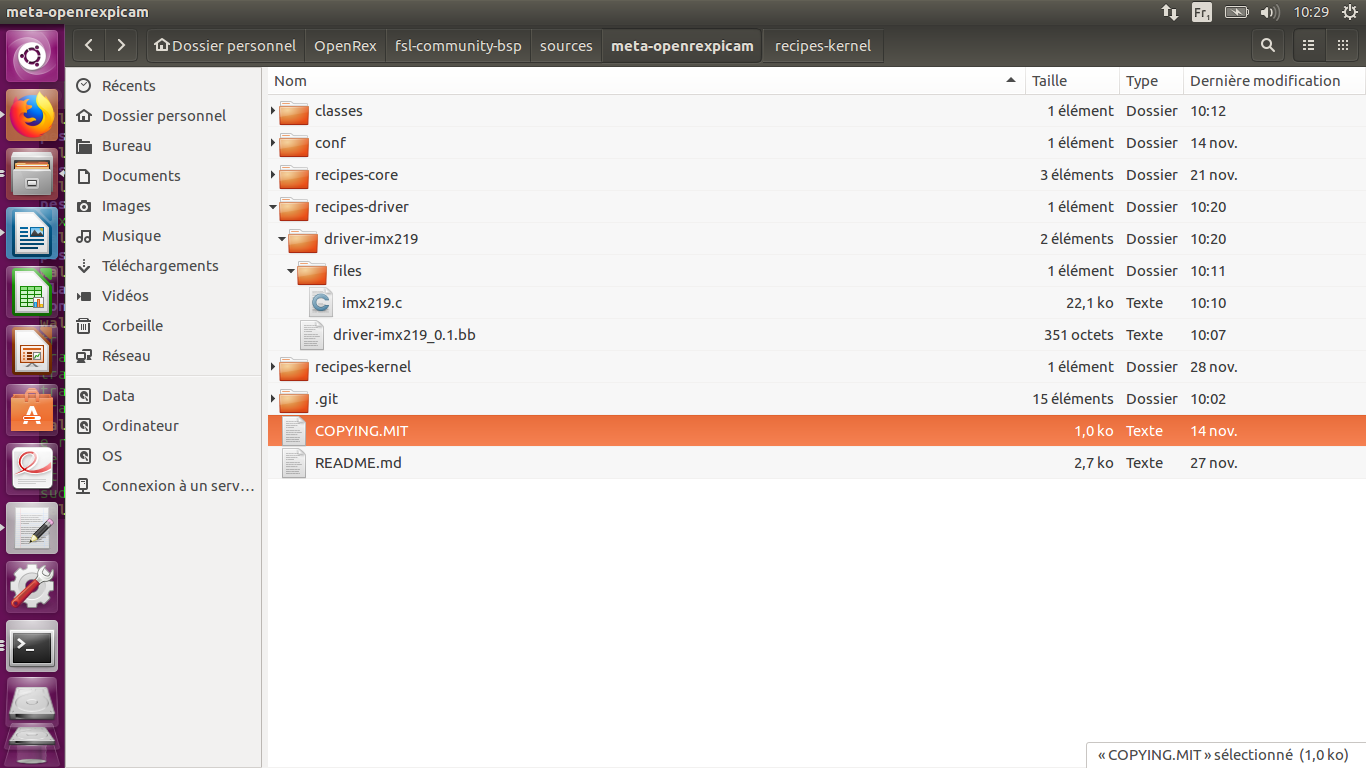
\includegraphics[width=1\linewidth,trim={9,5cm 14,5cm 15cm 6,7cm},clip]{arborescence.png}
    \decoRule
    \caption{Arborescnce des fichiers}  \label{fig:arbor}
\end{figure}

\section{Compilation de driver}
Extrait de la recette : récupère le fichier imx219.c, le compile par la cross
tool-chain et l’installe

\begin{lstlisting}
SUMMARY = "driver imx219"
SECTION = "examples"
LICENSE = "MIT"
LIC_FILES_CHKSUM = "file://${COMMON_LICENSE_DIR}/MIT;md5=c2b5f7071fdde268bf46ace1546f3c4b"

SRC_URI = "file://imx219.c"

S = "${WORKDIR}"

do_compile() {
         ${CC} imx219.c -o imx219
}

do_install() {
         install -d ${D}${bindir}
         install -m 0755 imx219 ${D}${bindir}
}
\end{lstlisting}

\section{Utilisation du driver sur la cible}
Vérification de la présence du driver dans l’arborescence :

\begin{figure}[th]
    \centering
    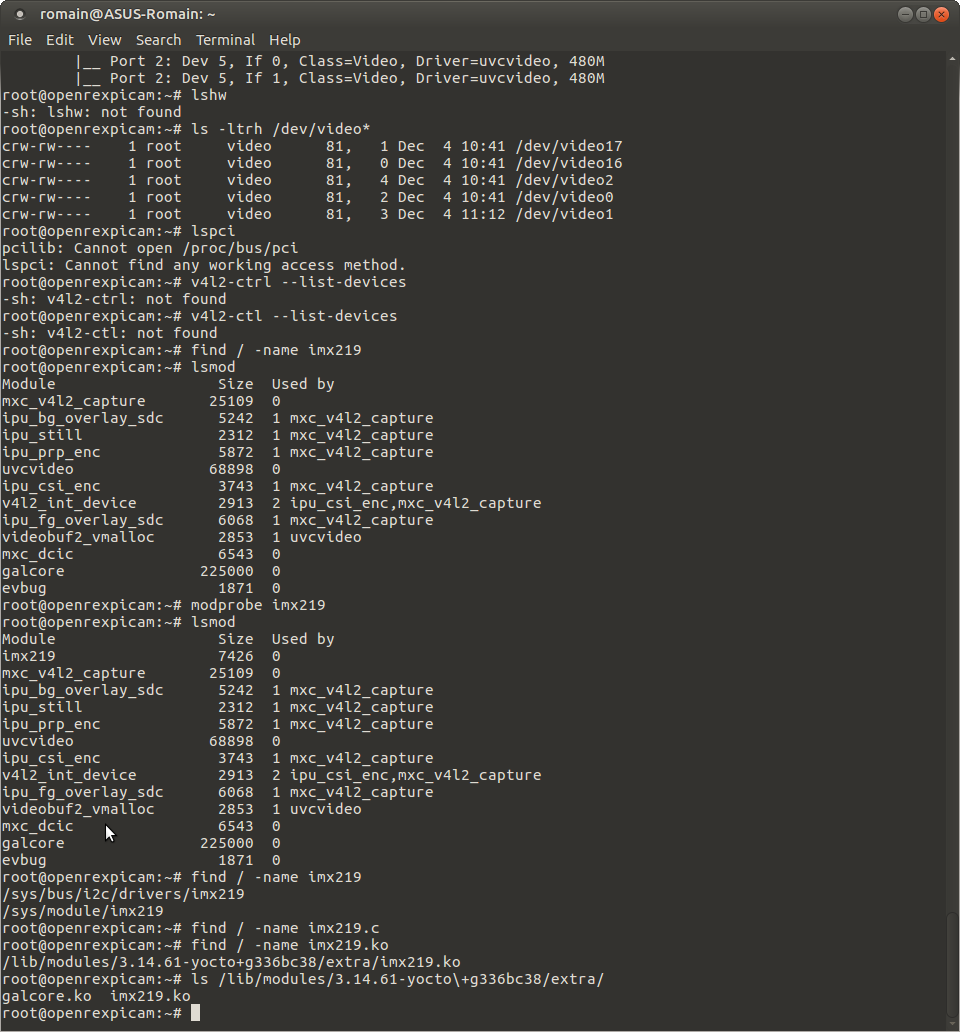
\includegraphics[width=1\linewidth,trim={0cm 1cm 0cm 33,1cm},clip]{presence.png}
    \decoRule
    \caption{Vérification de la présence du driver}  \label{fig:pres}
\end{figure}

Chargement du module imx219 :

\begin{figure}[th]
    \centering
    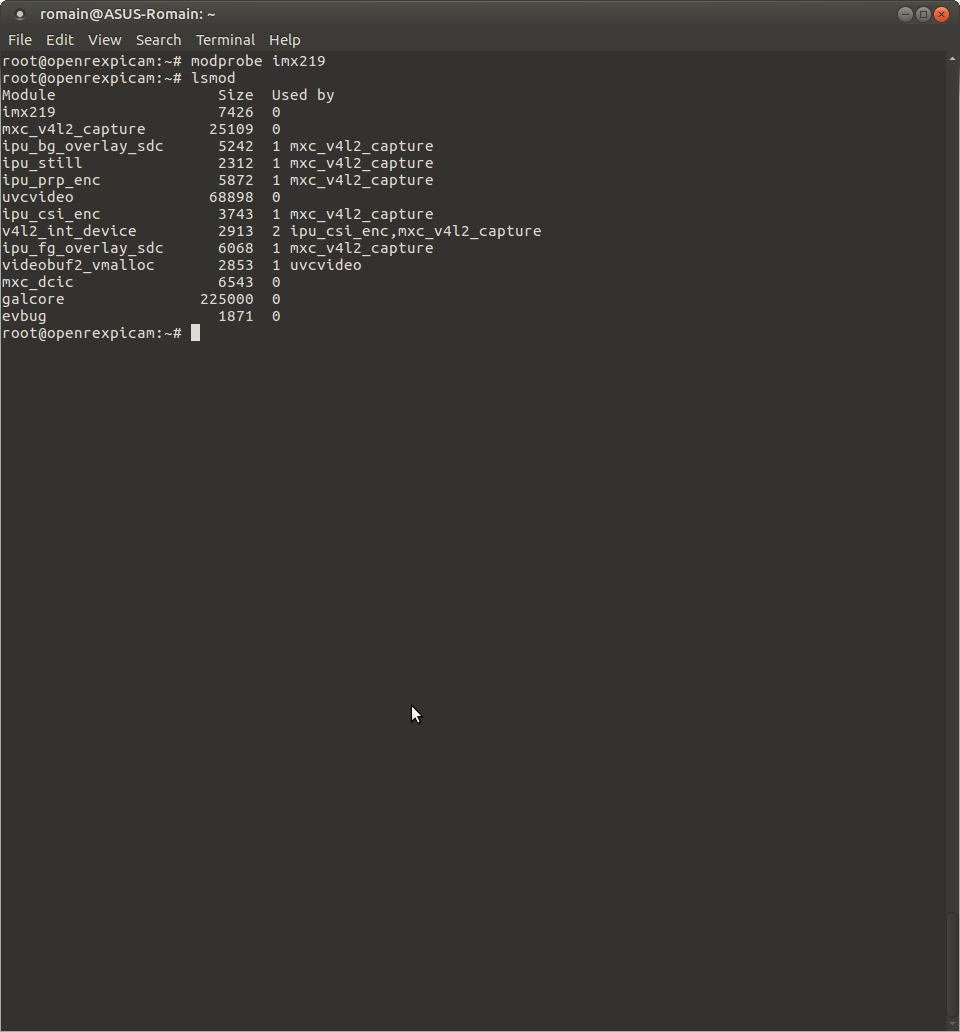
\includegraphics[width=1\linewidth,trim={0cm 25cm 0cm 1,8cm},clip]{module.png}
    \decoRule
    \caption{Chargement du module}  \label{fig:mod}
\end{figure}

Comme nous pouvons le voir le driver n’est pas encore utilisé par v4l (Used by 0).

\clearpage

Chargement du module à l’adresse I2C de l’imx219 :

\begin{figure}[th]
    \centering
    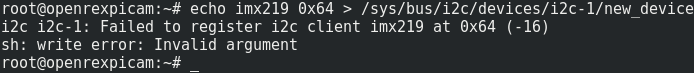
\includegraphics[width=1\linewidth]{modadd.png}
    \decoRule
    \caption{Chargement du module avec l'adresse I2C}  \label{fig:modadd}
\end{figure}

Erreur sur le bus i2c sur laquelle nous travaillons actuellement.
Récupération du flux vidéo en local via Gstreamer :

\textbf{\# gst-launch-1.0 v4l2src device="/dev/videoX" ! video/x-raw,width=640,height=480 ! autovideosink}

X’ étant le numéro correspondant au numéro du driver vidéo du port CSI-2

Actuellement nous cherchons l’utilisation des commandes gst-launch-1.0 et des
fichiers de configurations v4l2src (cf. Chapitre \ref{Chapter5}).

\section{Conclusion}

Cette solution est notre piste la plus concrète. En effet la compilation a réussi,
nous cherchons à comprendre comment utiliser le driver à travers v4l. Une fois cette
tache effectuée nous travaillerons sur le portage des versions du kernel (3.14 $\rightarrow$ 4.1).

%----------------------------------------------------------------------------------------

% Chapter 4

\chapter{Conclusion} % Main chapter title

\label{Chapter4} % For referencing the chapter elsewhere, use \ref{Chapter4} 

%----------------------------------------------------------------------------------------

\section{Bilan technique (AA,ML)}

\begin{table}[htp]
    \centering
    \begin{tabular}{|p{0.6\textwidth}|p{0.15\textwidth}|}
        \hline
        Mise en place d'un environnement de compilation & Terminé \\ \hline
        Développement d'un OS bootable sur l'OpenRex & Terminé \\ \hline
        Driver imx219 & En cours \\ \hline
    \end{tabular}
    \caption{Conclusion du projet} \label{tab:conclusion} 
\end{table}

Au cours du projet, nous somme tombés sur plusieurs impasses qui nous ont permis
d’apprendre les différentes façons de compiler un driver avec Yocto. \medskip

De part notre faible connaissance en driver Linux, nous ne pensions pas avoir les
capacités techniques requises pour développer nous-même un driver. Notre travail c’est
donc orienté vers trois drivers imx219 existants. Le BSP Openrex étant compatible avec le
kernel 3,14 et 4,1 nous étions limités en ressources. Deux des drivers n’était pas
compatible avec notre kernel, nous avons alors cherché à déterminer quelles
bibliothèques étaient responsable de cette incompatibilité. Malheureusement, les versions
étaient trop éloignées pour imaginer patcher toutes les bibliothèques utiles au
fonctionnement des drivers.\medskip

Une dernière solution était de rendre compatible le driver avec notre kernel, après l’avoir
rendu compatible avec notre device tree nous avions un segmentation fault lors du chargement
du kernel. Simultanément nous portions le bsp de l’openrex sur un kernel 4.14 qui n’a pas pu être
testé suite à une erreur survenue avec le bootloader.\medskip

Face à ces multiples échecs et un échange avec le client, nous commencions à rédiger
notre propre driver en se basant sur ceux déjà inclus dans le kernel. Le driver est
maintenant compilé et configuré par le device tree cependant il nous est impossible de lire
ou d’écrire dans un registre de la carte. Notre travaille s’achève donc sur ce point.\medskip

Techniquement nous avons acquis un bagage de connaissances concernant l’usage des
couches applicatives v4l2 nécessaire à la capture d’images de l’environnement Yocto. À
l’issue de ce rapport, nous pouvons nous concentrer sur le développement du code en
langage C.

\section{Bilan de suivi de projet (AA,ML)}

Dès le commencement du projet, nous somme partis en méthode agile, notre groupe de
travail a su s’auto-organiser et a perduré jusqu’à la fin du temps imparti. Nous avons
rapidement et facilement réussi à répartir le travail en fonction des compétences de
chacun, des obstacles matériels et logistiques rencontrés. \medskip

Malgré les différences de niveaux initials dûes au passif technologique de chacun, chaque individu
à apporter son utilité. En revanche, si le côté, communication et adaptabilité de la méthode agile
est respecté, le lien avec le client quant à lui a été négligé. \medskip

C’est en partie dû à la séparation physique du scrum-master et du groupe puis au manque d’outils
mise en place pour faciliter ce rapprochement. Une communication plus efficace avec l’équipe de
Thales nous aurait évité par exemple de prolonger trop longtemps la piste des drivers existants.

\section{Conclusion (AA,ML)}

Nous n’avons pas pu répondre complètement à la demande de Thales, qui est
actuellement entrain de développer le driver avec des résultats encouragent. Face au
obstacle notre groupe a toujours cherché à progresser en allant de plus en plus loin dans
le raisonnement technique. Bien quinachevé, cette expérience reste une des plus
enrichissantes de notre année. Étant soucieux d’apporter notre pierre à l’édifice nous
laissons avec ce rapport un environnement de développement Yocto optimisé pour
compiler un OS compatible avec l’Openrex et un guide d’utilisation et de développement
en annexe. 
%% Chapter 5

\chapter{État de l'art de la récupération du flux vidéo} % Main chapter title

\label{Chapter5} % For referencing the chapter elsewhere, use \ref{Chapter5}

%----------------------------------------------------------------------------------------

\section{Methodologie par la Webcam USB}

Nous nous aguérissons à l’utilisation de Video4Linux-utils, de plus nous avons trouvé
un journal en ligne expliquant la récupération du flux vidéo d’une webcam USB avec
V4L2-utils sur imx6. Dans un premier temps, nous avons capturé le flux d’une
webcam USB intégrée à un de nos ordinateurs personnels afin de comprendre les commandes
et paramètres. Ensuite nous avons récupéré une webcam USB lambda afin de tester les commandes
sur la carte openrex et essayer de capturer le retour vidéo. Une fois fonctionnel
nous passerons sur le flux vidéo de la Raspi Cam v2.

% \section{Commandes}
\begin{enumerate}
  \item Récupérer le port qui est connecté la webcam USB grâce à la commande :
  \textbf{lsusb -t}
\begin{figure}[th]
    \centering
    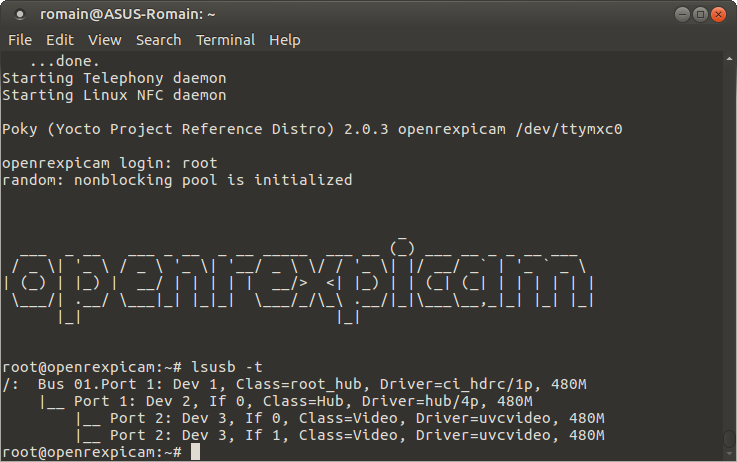
\includegraphics[width=1\linewidth,trim={0cm 0,6cm 0cm 12,5cm},clip]{webcam1.png}
    \decoRule
    \caption{Port USB de la webcam USB}  \label{fig:webcam1}
\end{figure}

\item La webcam USB est sur le bus I2C n°1 avec comme identifiant de port 1.2.
\begin{figure}[th]
    \centering
    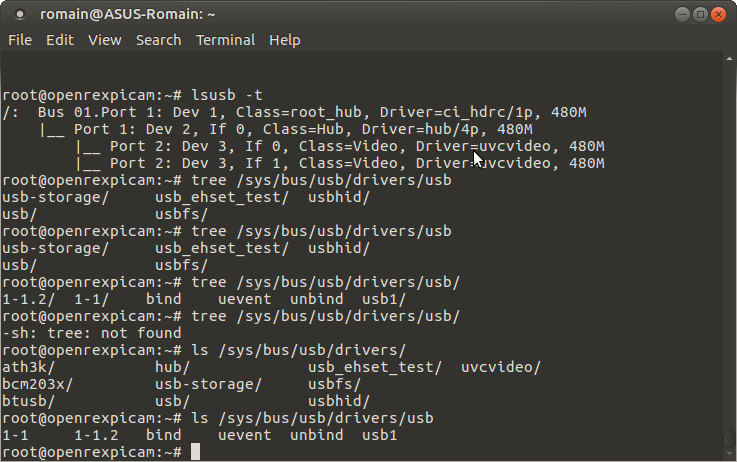
\includegraphics[width=1\linewidth,trim={0cm 0,6cm 0cm 14,5cm},clip]{webcam2.png}
    \decoRule
    \caption{Vérification du port et identifiant de la webcam USB}  \label{fig:webcam2}
\end{figure}

\item Il est nécessaire d'écrire le numéro du bus et l’identifiant du port dans les fichiers bind
et unbind. Le fichier bind permet de  « lier » un appareil USB à son driver et
ainsi le rendre visible pour le système tandis que le fichier unbind lui détache
le driver de son appareil USB pour le « cacher » du système.
\begin{figure}[th]
    \centering
    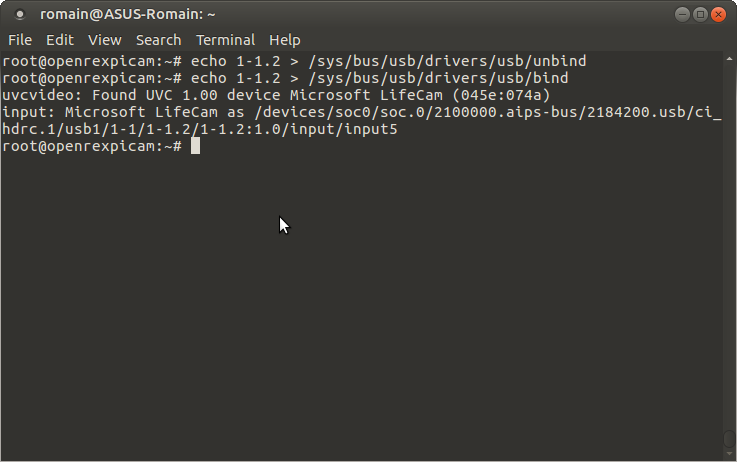
\includegraphics[scale=0.5,trim={0cm 11,5cm 0cm 1,9cm},clip]{webcam3.png}
    \decoRule
    \caption{Liaison entre la webcam USB et son driver}  \label{fig:webcam3}
\end{figure}

\item La webcam USB est bien reconnu par notre système qui affiche sa
référence (cf. Figure \ref{fig:webcam3}).

\item Démarrer un flux vidéo sur notre webcam USB s'effectue avec la commande :
\textbf{\# gst-launch-1.0 v4l2src device="/dev/video0" ! video/x-raw,w
idth=640,height=480 ! autovideosink}

\begin{figure}[th]
    \centering
    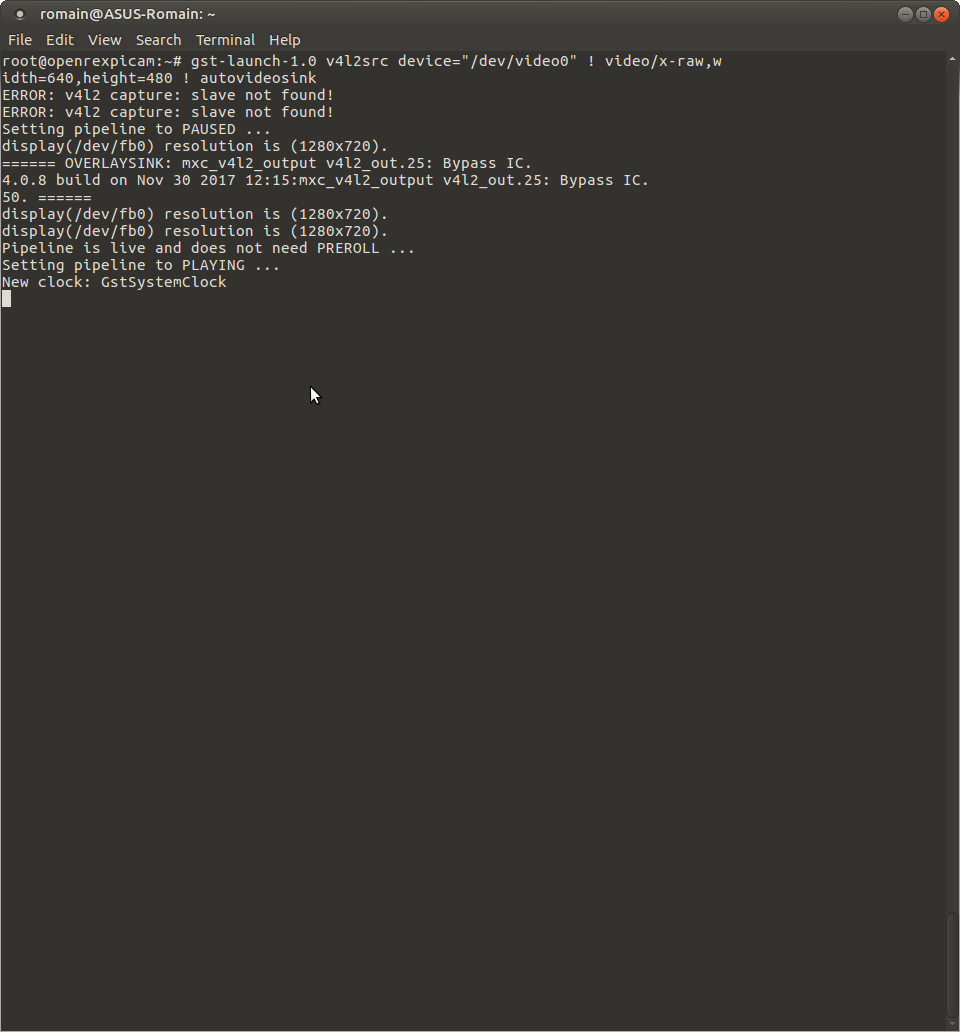
\includegraphics[scale=0.4,trim={0cm 26,1cm 0cm 1,7cm},clip]{webcam4.png}
    \decoRule
    \caption{Capture du flux vidéo de la webcam USB}  \label{fig:webcam4}
\end{figure}

\item Nous sommes persuadés de la bonne capture du flux vidéo puisque lorsque
nous la lançons, le retour de la commande se fige à :

\begin{lstlisting}
New clock GstSystemClock
\end{lstlisting}

C'est exactement le même endroit quand nous lançons la même commande sur notre
propre ordinateur avec notre webcam intégrée. De plus une petite LED verte s’allume
au moment de l’envoi de cette commande (cf. Figure \ref{fig:webcam5}).
\begin{figure}[th]
    \centering
    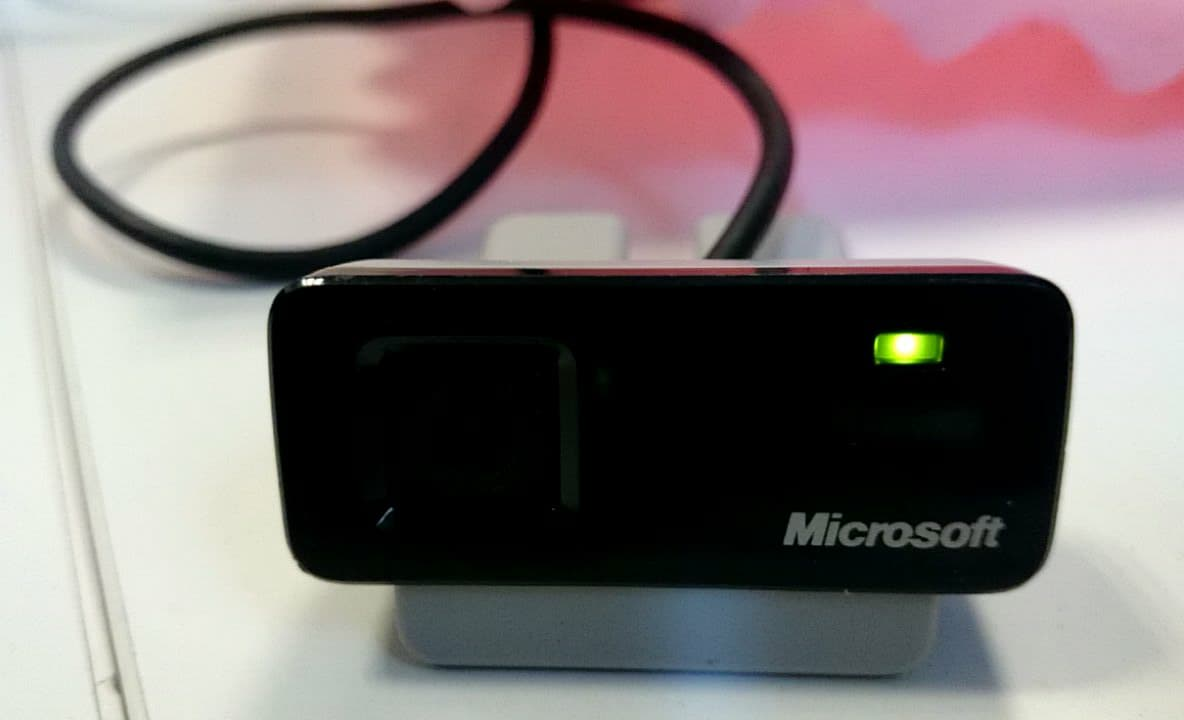
\includegraphics[scale=0.15,trim={10cm 2cm 4cm 9,5cm},clip]{webcam5.png}
    \decoRule
    \caption{LED verte allumée lors de l'envoi de la commande}  \label{fig:webcam5}
\end{figure}

\end{enumerate}

\section{Problèmes}

Notre principal problème pour l’instant est de récupérer ce flux vidéo puisqu’il
est impossible de l’afficher directement dans le terminal, pour tester cela nous
essayons de l’afficher sur nos ordinateurs par le réseau WiFi en protocole UDP.

\section{Point d'amélioration}

Pour commencer il est nécessaire de mettre l’image de l'openrex à jour afin de se
connecter à un réseau WiFi ensuite récupérer ce flux vidéo par le réseau WiFi sur
nos ordinateurs en UDP.

Finalement une fois que nous aurons réussi à afficher le flux vidéo de la webcam
USB sur nos ordinateurs nous essayerons d’effectuer le même processus mais pour
la Raspi Cam v2, qui se pilote par le CSI et non l’USB.

\section{Sources}

Lien du blog de la récupération du flux vidéo par la webcam USB : 

\href{http://jas-hacks.blogspot.fr/2014/04/imx6-gstreamer-imx-and-usb-webcam.html}
{http://jas-hacks.blogspot.fr/2014/04/imx6-gstreamer-imx-and-usb-webcam.html}
 

%----------------------------------------------------------------------------------------
%	THESIS CONTENT - APPENDICES
%----------------------------------------------------------------------------------------

%\appendix % Cue to tell LaTeX that the following "chapters" are Appendices

% Include the appendices of the thesis as separate files from the Appendices folder
% Uncomment the lines as you write the Appendices

%
\section{Procédure initiale}
Cette partie sera une explication des différentes commandes ainsi qu’une description de la
méthodologie choisie pour travailler avec Yocto.
\subsection{Gérer son espace mémoire}

Tout d’abord sachons que le manuel Yocto conseille de réserver 50 Go afin
de pouvoir travailler dans de bonnes conditions. Dans notre cas nous avons une
partition de 100 Go incluant Ubuntu14 (5 Go), à terme notre répertoire de
travail sera suffisamment agrandi pour combler les 40 Go.
Pour ne pas trop encombrer son espace de stockage on peut définir dans build/local.conf la variable

\begin{lstlisting}
INHERIT += "rm_work" //effacera les fichiers intermédiaires au fur et a mesure
RM_OLD_IMAGE = "1" //remplacera les images par la plus récente.
\end{lstlisting}

Attention ces variables vous feront perdre des données, rm\_work par exemple
libérera de l'espace (16Go) mais rendra impossible le débogage de la compilation.
La suppression des images précédentes est conseillée quand on est amené à en
générer beaucoup. Une image pèse quelques centaines de Mo.
\subsection{Préparation de l’environnement}
Packages requis pour une compilation Yocto :

\begin{itemize}
	\item[-] Git 1.8.3.1 ou plus
	\item[-] Tar 1.27 ou plus
	\item[-] Python 3.4.0 ou plus
\end{itemize}

\begin{tcolorbox}
	user@poky:~\$ sudo apt-get install gawk wget git-core diffstat unzip texinfo gcc-multilib \
	build-essential chrpath socat cpio python python3 python3-pip python3-pexpect \
	xz-utils debianutils iputils-ping libsdl1.2-dev xterm repo
\end{tcolorbox}

\subsection{Téléchargement des sources Freescale}
La première étape consiste à télécharger tous les exécutables et métadonnées nécessaires pour créer l’image de base de l’OpenRex. En premier lieu il est nécessaire de récupérer la commande repo via les dépots officiels ou téléchargement :

\begin{tcolorbox}
	sudo aptitude install repo
	sudo aptitude update
	sudo aptitude upgrade
\end{tcolorbox}

ou

\begin{tcolorbox}
	mkdir bin
	curl http://commondatastorage.googleapis.com/git-repo-downloads/repo > bin/repo
	chmod a+x bin/repo
	PATH=\${PATH}:bin
\end{tcolorbox}

Ensuite il faut créer le répertoire de travail :

\begin{tcolorbox}
	mkdir fsl-community-bsp \&\& cd fsl-community-bsp
	\subsubsection{Yocto version 2.0}
	Création du répertoire du fichier manifest :
\end{tcolorbox}

\begin{tcolorbox}
	mkdir -p ./repo/local\_manifests/
\end{tcolorbox}

Télécharger l’ensemble des sources externes de ce projet par la commande

\begin{tcolorbox}
	repo init -u https://github.com/Freescale/fsl-community-bsp-platform -b jethro
\end{tcolorbox}

De plus il Noter le manifest pour pouvoir télécharger/installer/décompresser les sources produites par Fedevel.

\begin{tcolorbox}
	cat > .repo/local\_manifests/imx6openrex.xml << EOF
	<?xml version="1.0" encoding="UTF-8"?>
	<manifest>
	<remote fetch="git://github.com/FEDEVEL" name="fedevel"/>
	<project remote="fedevel" revision="jethro" name="meta-openrex" path="sources/meta-openrex\">
	<copyfile src="openrex-setup.sh" dest="openrex-setup.sh"/>
	</project>
	</manifest>
	EOF
\end{tcolorbox}

Enfin, il est nécessaire de télécharger/installer/décompresser ces fichiers :

\begin{tcolorbox}
	repo sync
\end{tcolorbox}

\subsubsection{Yocto version 2.1}
\begin{tcolorbox}
	repo init -u git@github.com/petit-romain/fsl-community-bsp-platform.git
\end{tcolorbox}

Enfin, il est nécessaire de télécharger/installer/décompresser ces fichiers :

\begin{tcolorbox}
	repo sync
\end{tcolorbox}

\subsection{Compilation ( Yocto 2.0 )}
Créer et sourcer l'environnement pour que la compilation inclut la métadonnée Openrex.

\begin{tcolorbox}
	source openrex-setup.sh
\end{tcolorbox}

Préparer l’environnement et construire l’image. Toutes Les commandes ci-dessous seront à effectuer pendant l’usage courant, elles ne font plus vraiment partie de l’initialisation du projet.


\begin{tcolorbox}
	MACHINE=imx6s-openrex source setup-environment build-dir
	bitbake core-image-base
\end{tcolorbox}

\subsection{Compilation ( Yocto 2.1 )}

\begin{tcolorbox}DISTRO=poky MACHINE=imx6-openrexbasic source setup-environment build-dir
	bitbake openrexpicam-base-image
\end{tcolorbox}

\subsection{Déploiement de l’image ( Yocto 2.0 )}

Installer l’image sur la carte-sd

\begin{tcolorbox}
	umount /dev/YourSDCard

	gunzip -c tmp/deploy/images/imx6s-openrex/core-image-base-imx6s-openrex.sdcard.gz > tmp/deploy/images/imx6s-openrex/core-image-base-imx6s-openrex.sdcard
	sudo dd if=tmp/deploy/images/imx6s-openrex/core-image-base-imx6q-openrex.sdcard of=/dev/YourSDCard
	umount /dev/YourSDCard
\end{tcolorbox}

A présent insérez la carte sd dans l’OpenRex et démarrez, vous devriez voir l’autoboot apparaître grâce à la communication série.

\subsection{Déploiement de l’image ( Yocto 2.1 )}

\begin{tcolorbox}
	umount /dev/YourSDCard
	gunzip -c tmp/deploy/images/imx6-openrexbasic/core-image-base-imx6-openrexbasic.sdcard.gz > build-openrex/tmp/deploy/images/imx6-openrexbasic/core-image-base-imx6-openrexbasic.sdcard
	sudo dd if=tmp/deploy/images/imx6-openrexbasic/core-image-base-imx6-openrexbasic.sdcard of=/dev/YourSDCard
	umount /dev/YourSDCard
\end{tcolorbox}

Si vous obtenez l’erreur "Error : bootmmc not defined " , redémarrez l’OpenRex et interrompez le boot de celle-ci afin de lancer la commande ci dessous :

\begin{tcolorbox}
	setenv bootmmc "run findfdt; mmc dev \${mmcdev}; if mmc rescan; then if run loadbootscript;
	then run bootscript; else if run loadimage; then run mmcboot; else run netboot;
	fi; fi; else run netboot; fi;\textbackslash0"; saveenv; reset;
\end{tcolorbox}

\subsection{Etat initial}
Une fois la procédure faite, on doit retrouver les fichiers suivant dans le
dossier fsl-community-bsp :
\begin{itemize}
	\item[fsl-setup-release.sh :] script déjà utilisé à la premère préparation
	de l’environnement.
	\item[setup-environment :] est utilisé pour sourcer les variables d'environnement
	utiles lors de la création de l'image.
	\item[Build-dir :] contient tous les fichiers générés lors des compilations.
	On y trouve :
	\item[bitbake.lock :] sémaphore temporaire assurant qu’une seule instance de bitbake
	accède aux fichiers
	\item[cache :]
	\item[conf :]
	\item[sstate-cache :] avantage majeur de Yocto sur des compilation standard, dans ce répertoire sont stockées les états de compilation intermédiaire de Yocto. Pour vider la shared state cache on lance :]
	\begin{tcolorbox}
		bitbake <recette> -c cleansstate.
	\end{tcolorbox}

	\item[tmp :] dossier principal de compilation, tmp/work contient les sources des recettes et tmp/deploy les images
	\item[sources :] contient l'ensemble des     métas nécessaires à la création de l'image. On y trouve :]
	\item[meta-freescale :] configure l’image pour un processeur Freescale.
	\item[meta-fsl-arm :] configure l'image pour un cortex arm Freescale.
	\item[meta-fsl-arm-extra :] configure plus encore l'image pour un cortex arm Freescale.
	\item[meta-fsl-bsp-release :] configure l’image pour une carte officielle à processeur Freescale.
	\item[meta-fsl-arm-voipac :] surcouche des metas précédentes pour l’Openrex.
	\item[meta-openembedded :] contient les meta des drivers materiel tel que le bluetooth et les bibliothèques utiles a l'utilisation d’un driver par exemple le python.
	\item[meta-fsl-demos :] des démonstrations Freescale.
	\item[meta-browser :] permet d’avoir mozilla ou bien chrome sur l’image.
	\item[poky :] contient la base du build system et les metadata de base relatif a la distribution.
	\item[base :] une base pour configurer son dossier build pour les meta Freescale.
	\item[meta-qt5 :] elle nous permet d'utiliser du code Qt par l’OpenRex en utilisant un SDK. (adresse pour le clonage :https://github.com/meta-qt5/meta-qt5.git)

	\subsection{Ajout de notre méta (Yocto 2.0)}
	\item[meta-openrexpicam:] la méta qui va définir notre distribution.        (https://github.com/Alanaitali/meta-openrexpicam.git)
	Si vous utilisez Yocto 2.0, notre meta doit simplement être copiée dans le dossier sources puis indiquée dans le bblayers.conf comme expliqué dans « Usage courant » ci-dessous. (follow me)
\end{itemize}

\begin{tcolorbox}
	cd \$BUILDDIR/../sources/.
	git clone https://github.com/Alanaitali/meta-openrexpicam.git
\end{tcolorbox}

\section{Usage courant}
Préparation de l’environnement
L’environnement de développement a été créé avec fsl-setup-release.sh, mais pour chaque terminal de travail, il faudra sourcer l’environnement à nouveau. C’est-à-dire ajouter des variables d’environnement qui seront nécessaire lors de la compilation. La commande suivante source l’environnement et dans le même temps nous lui indiquons le nom de la machine dans notre cas « imx6s-Openrex » que l’on retrouve dans les sources téléchargées. De cette manière nous donnons des paramètres qui seront pris en compte lors de la compilation avec le « bitbake ». Cette assignation de machine sera inscrite dans le local.conf de manière plus pérenne.

\subsubsection*{Yocto 2.0 :}


\begin{tcolorbox}
	MACHINE=imx6s-openrex source setup-environment build-dir
	bitbake core-image-base
\end{tcolorbox}

\subsubsection*{Yocto 2.1 :}

\begin{tcolorbox}
	DISTRO=poky MACHINE=imx6-openrexbasic source setup-environment build-dir
\end{tcolorbox}

\subsection{Vérification de l’image demandée}
Avant de lancer la compilation nous devons indiquer le chemin d’accès et
le nom des métadonnées à prendre en compte pour la compilation. Ces paquets
sont aussi appelés couches (layers), ils sont référencés dans le fichier
bblayer.conf dans le dossier /build-dir/conf. Pour inclure une nouvelle meta
à la compilation il faut écrire son chemin sur bblayers.conf.

\begin{lstlisting}
POKY_BBLAYERS_CONF_VERSION = "2"

BBPATH = "\${TOPDIR}"
BSPDIR := "\${@os.path.abspath(os.path.dirname(d.getVar('FILE', True)) + '/../..')}"
BBFILES ?= ""

BBLAYERS = " \
\${BSPDIR}/sources/poky/meta \
\${BSPDIR}/sources/poky/meta-poky \
\
\${BSPDIR}/sources/meta-openembedded/meta-oe \
\${BSPDIR}/sources/meta-openembedded/meta-multimedia \
\
\${BSPDIR}/sources/meta-fsl-arm \
\${BSPDIR}/sources/meta-fsl-arm-extra \
\${BSPDIR}/sources/meta-fsl-demos \
\
\${BSPDIR}/sources/meta-openrexpicam \
"
BBLAYERS += "\${BSPDIR}/sources/meta-fsl-arm-voipac"
\end{lstlisting}

Afin de configurer l’environnement de travail de bitbake on rédige un fichier local.conf. Attention à ce que le nom de machine (imx6-openrexbasic pour Yocto 2.1 et imx6s-openrex) soit en accord avec la recette utilisée.

\begin{lstlisting}
MACHINE ??= 'imx6-openrexbasic'
DISTRO ?= 'poky'
PACKAGE_CLASSES ?= "package_rpm"
EXTRA_IMAGE_FEATURES ?= "debug-tweaks"
USER_CLASSES ?= "buildstats image-mklibs"
PATCHRESOLVE = "noop"
BB_DISKMON_DIRS = "\
STOPTASKS,\${TMPDIR},1G,100K \
STOPTASKS,\${DL_DIR},1G,100K \
STOPTASKS,\${SSTATE_DIR},1G,100K \
STOPTASKS,/tmp,100M,100K \
ABORT,\${TMPDIR},100M,1K \
ABORT,\${DL_DIR},100M,1K \
ABORT,\${SSTATE_DIR},100M,1K \
ABORT,/tmp,10M,1K"
PACKAGECONFIG_append_pn-qemu-native = " sdl"
PACKAGECONFIG_append_pn-nativesdk-qemu = " sdl"
CONF_VERSION = "1"

DL_DIR ?= "\${BSPDIR}/downloads/"
ACCEPT_FSL_EULA = "1"
\end{lstlisting}

Par soucis de personnalisation la distribution du projet peut être renommée et le nombre de threads configurés en ajoutant :

\begin{lstlisting}
DISTRO ?= 'name'
BB_NUMBER_THREADS?="4"
PARALLEL_MAKE?="-j4"
\end{lstlisting}
\subsection{Compilation}

L’étape compilation prend bien moins de temps lors de l’usage régulier (près
de 24 fois plus rapide). Pendant cette étape nous avons un grand nombre
d’informations qui s’affichent sur le terminal, les plus importantes sont les
warnings et les erreurs de compilation qu’il est nécessaire de comprendre puis
interpréter pour résoudre.

\begin{tcolorbox}
	bitbake openrexpicam-base-image
\end{tcolorbox}

Une fois cette étape terminée on peut retrouver toutes une arborescence de dossier et de fichiers dans le dossier de construction (/build-dir), ces derniers seront au cœur du fonctionnement de notre appareils. ils sont spécifiques à notre carte, les modules, les capteurs qu’elle comporte. Le fruit de la compilation de l’image contient le root-filesystem le kernel le bootloader et le device-tree en un seul fichier compressé. /build-dir/tmp/deploy/images/imx6-openrexbasic doit contenir :

\begin{itemize}
	\item[1 image sous format] .sdcard.gz
	\item[1 image sous format] .rootfs.ext4
	\item[1 image sous format] .rootfs.manifest
	\item[1 image sous format] .rootfs.sdcard
\end{itemize}

%\include{Appendices/AppendixB}
%\include{Appendices/AppendixC}

%----------------------------------------------------------------------------------------
%	BIBLIOGRAPHY
%----------------------------------------------------------------------------------------

%\printbibliography[heading=bibintoc]

%----------------------------------------------------------------------------------------

\end{document}  
